\section{Controlando confundidores (critério \textit{backdoor})}
\label{sec:backdoor}

Um confundidor é uma causa comum, 
direta ou indireta, de $X$ em $Y$.
Na existência de confundidores,
a regressão de $Y$ em $X$ no modelo observacional, 
$\E[Y|X]$, é diferente desta regressão
no modelo de intervenção, $\E[Y|do(X)]$.
Isto ocorre pois, quando calculamos $\E[Y|X]$,
utilizamos toda a informação em $X$ para prever $Y$.
Esta informação inclui não apenas 
o efeito causal de $X$ em $Y$, como 
também a informação que $X$ traz indiretamente sobre $Y$ 
pelo fato de ambas estarem associados aos seus confundidores.

Para ilustrar este raciocínio, 
podemos revisitar o \cref{ex:simpson_fim}.
uma vez que Sexo (Z) é causa comum do Tratamento (X) e
da Cura (Y), Z é um confundidor.
Quando calculamos $f(y|x)$ (\cref{eq:prob_causa_1}), 
utilizamos não só o efeito direto de $X$ em $Y$, 
expresso em $f(y|x,z)$, como também 
a informação que indireta que $X$ traz sobre $Y$
por meio do confundidor $Z$,
expressa pela combinação de $f(z|x)$ com $f(y|x,z)$.

Esta seção desenvolve uma estratégia para
medir o efeito causal chamada de 
critério \textit{backdoor}, que
consiste em bloquear 
todos os caminhos de informação que passam por confundidores:

\begin{definition}
 \label{def:backdoor}
 Seja $\sG = (\sV, \sE)$ um grafo causal e $X, Y \in \sV$.
 Dizemos que $\Z \subseteq \sV - \{X,Y\}$ satisfaz 
 o critério ``backdoor'' se:
 \begin{enumerate}
  \item $X \notin Anc(\Z)$,
  \item Para todo caminho de $X$ em $Y$, 
  $C = (X, C_2, \ldots, C_{n-1}, Y)$ tal que
  $(C_2, X) \in \sE$, $C$ está bloqueado dado $\Z$.
 \end{enumerate}
\end{definition}

\begin{example}
 No \cref{ex:simpson_fim} o único caminho de $X$ em $Y$ em que
 o vértice ligado a $X$ é pai de $X$ é $X \leftarrow Z \rightarrow Y$.
 Como $Z$ é um confudidor neste caminho, ele o bloqueia.
 Assim, $Z$ satisfaz o critério backdoor.
\end{example}

\begin{example}
\begin{knitrout}
\definecolor{shadecolor}{rgb}{0.969, 0.969, 0.969}\color{fgcolor}\begin{figure}[t]

{\centering 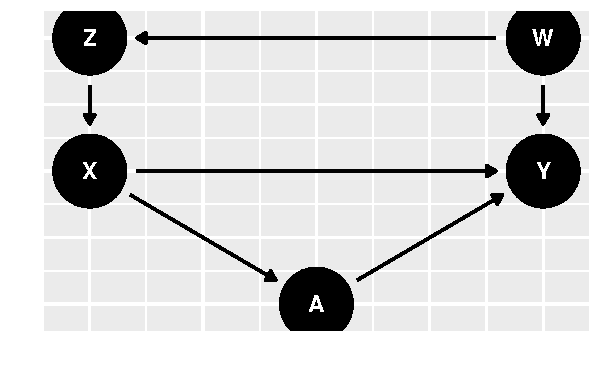
\includegraphics[width=\maxwidth]{figure/backdoor_ex_1-1} 

}

\caption[Para medir o efeito causal de X em Y, podemos aplicar o critério backdoor]{Para medir o efeito causal de X em Y, podemos aplicar o critério backdoor. Neste grafo o único caminho aplicável ao critério backdoor é (X, Z, W, Y). Neste caminho, $Z$ é uma cadeia e $W$ é um confundidor. Assim, todas as possibilidades dentre Z, W, (Z,W) bloqueiam o caminho e satisfazem o critério backdoor.}\label{fig:backdoor_ex_1}
\end{figure}

\end{knitrout}

 Considere o grafo causal na \cref{fig:backdoor_ex_1}.
 Para aplicar o critério backdoor, devemos identificar
 todos os caminhos de $X$ em $Y$ em que
 o vértice ligado a $X$ é pai de $X$, isto é,
 temos $X \leftarrow$. O único caminho deste tipo é:
 $X \leftarrow Z \leftarrow W \rightarrow Y$.
 Neste caminho, $Z$ é uma cadeia e $W$ é um confudidor.
 Assim, é possível bloquear este caminho condicionando
 em $Z$, em $W$, e em $(Z,W)$.
 Isto é, todos estas combinações 
 satisfazem o critério backdoor.
\end{example}

\begin{example}
\begin{knitrout}
\definecolor{shadecolor}{rgb}{0.969, 0.969, 0.969}\color{fgcolor}\begin{figure}[t]

{\centering 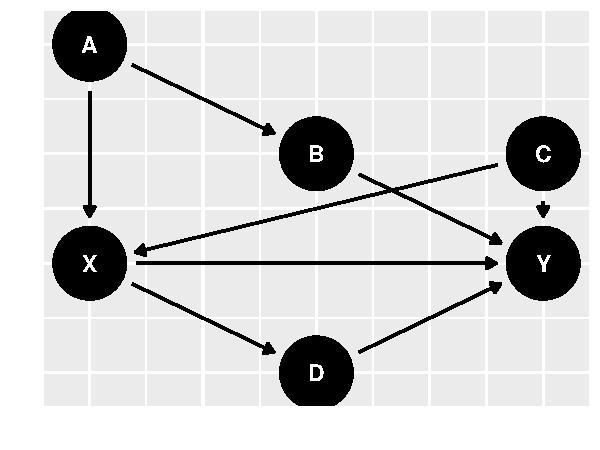
\includegraphics[width=\maxwidth]{figure/backdoor_ex_2-1} 

}

\caption[Para medir o efeito causal de X em Y, podemos aplicar o critério backdoor]{Para medir o efeito causal de X em Y, podemos aplicar o critério backdoor. Neste grafo existem dois caminhos aplicáveis ao critério backdoor: (X, A, B, Y) e (X, C, Y). No primeiro, A é um confundidor. No segundo caminho, C é um confudidor. Assim, (A,C) bloqueia ambos os caminhos e satisfaz o critério backdoor.}\label{fig:backdoor_ex_2}
\end{figure}

\end{knitrout}

 Considere o grafo causal na \cref{fig:backdoor_ex_2}.
 Para aplicar o critério backdoor,
 encontramos todos os caminhos de $X$ em $Y$ em que
 o vértice ligado a $X$ é pai de $X$. 
 Há dois caminhos deste tipo:
 $X \leftarrow A \rightarrow B \rightarrow Y$ e
 $X \leftarrow C \rightarrow Y$.
 Como $A$ e $C$ são confudidores, respectivamente,
 no primeiro e segundo caminhos, 
 $(A,C)$ bloqueia ambos eles.
 Assim $(A,C)$ satisfaz o critério backdoor.
 Você consegue encontrar outro conjunto de variáveis que
 satisfaz o critério backdoor?
 
 Também é possível identificar 
 os conjuntos de variáveis que satisfazem
 o critério backdoor por meio
 do pacote \textit{dagitty},
 como ilustrado a seguir:
 
\begin{knitrout}
\definecolor{shadecolor}{rgb}{0.969, 0.969, 0.969}\color{fgcolor}\begin{kframe}
\begin{alltt}
\hlkwd{library}\hlstd{(dagitty)}
\hlcom{# Especificar o grafo}
\hlstd{grafo} \hlkwb{<-} \hlkwd{dagitty}\hlstd{(}\hlstr{"dag\{
    X[e] Y[o]
    A -> \{ X B \}; B -> \{ Y \}; C -> \{ X Y \};
    X -> \{ D Y \}; D -> Y \}"}\hlstd{)}

\hlkwd{adjustmentSets}\hlstd{(grafo,} \hlkwc{type} \hlstd{=} \hlstr{"all"}\hlstd{)}
\end{alltt}
\begin{verbatim}
## { A, C }
## { B, C }
## { A, B, C }
\end{verbatim}
\end{kframe}
\end{knitrout}
\end{example}

O critério backdoor generaliza duas condições especiais que
são muito utilizadas.
Em uma primeira condição, 
o valor de $X$ é gerado integralmente por
um aleatorizador, independente de todas as demais variáveis.
Esta ideia é captada pela 
\cref{def:aleatorizacao}, abaixo:

\begin{definition}
 \label{def:aleatorizacao}
 Dizemos que $X$ é um experimento aleatorizado simples 
 se $X$ é ancestral.
\end{definition}

Em um experimento aleatorizado simples não há confundidores.
Assim, $\emptyset$ satisfaz o critério backdoor:

\begin{lemma}
 \label{lemma:backdoor_random}
 Se $X$ é um experimento aleatorizado simples, então
 $\emptyset$ satisfaz o critério backdoor.
\end{lemma}

Veremos que em um experimento aleatorizado simples a
distribuição intervencional é igual 
à distribuição observacional.
Assim, $\E[Y|do(X)] = \E[Y|X]$ e
a inferência causal é reduzida 
à inferência comumente usadas para
a distribuição observacional.

Além disso, o conjunto de todos os pais de $X$
também satisfaz o critério backdoor:

\begin{lemma}
 \label{lemma:backdoor_pais}
 $\Z = Pa(X)$ satisfaz o critério backdoor para
 medir o efeito causal de $X$ em $Y$.
\end{lemma}

A seguir, veremos como o critério backdoor permite
a identificação causal, isto é,
uma equivalência entre quantidades de interesse
obtidas pelo modelo de intervenção e
quantidades obtidas pelo modelo observacional.

\subsection{Identificação causal usando o critério backdoor}

A seguir, o \cref{thm:backdoor} mostra que,
se $\Z$ satisfaz o critério backdoor, então
é possível ligar algumas 
distribuições sob intervenção em $X$ a
distribuições observacionais:

\begin{definition}
 \label{def:conf_control}
 $\Z$ controla confundidores para
 medir o efeito causal de $X$ em $Y$ se
 \begin{align*}
  f(\z|do(x)) 
  &= f(\z), \text{ e } \\
  f(y|do(x), \z) 
  &= f(y|x, \z).
 \end{align*}
\end{definition}

\begin{theorem}
 \label{thm:backdoor}
 Se $\Z$ satisfaz 
 o critério backdoor para medir
 o efeito causal de $X$ em $Y$, então
 $\Z$ satisfaz a \cref{def:conf_control}.
\end{theorem}

O \cref{thm:backdoor} mostra que,
se $\Z$ satisfaz o critério backdoor, então
distribuição de $\Z$ quando
aplicamos uma intervenção em $X$ é igual
à distribuição marginal de $\Z$.
Além disso, a distribuição condicional de
$Y$ dado $\Z$ quando aplicamos uma intervenção em $X$ é igual 
à distribuição de $Y$ dado $X$ e $Z$.
Assim, o \cref{thm:backdoor} relaciona
distribuições que não geraram os dados a 
distribuições que os geraram.
Com base neste resultado, é possível determinar
$f(y|do(x))$ a partir de $f(y,x,\z)$:

\begin{corollary}
 \label{cor:backdoor}
 Se $\Z$ satisfaz
 a \cref{def:conf_control}, então
 \begin{align*}
  f(y|do(x)) &=
  \int f(y|x,\z)f(\z)d\z.
 \end{align*}
\end{corollary}

Para compreender intuitivamente o \cref{cor:backdoor},
podemos retornar ao \cref{ex:simpson_fim}.
Considere o caso em que $X, Y, Z$ são as indicadoras de que,
respectivamente, o paciente foi submetido ao tratamento,
se curou e, é de sexo masculino.
Similarmente ao \cref{thm:backdoor},
vimos em \cref{ex:simpson_fim} que $f(y|do(x))$ é
a média de $f(y|x,z)$ ponderada por $f(z)$.
Nesta ponderação, utilizamos $f(z)$ 
ao invés de $f(z|x)$ pois $Z$ é um confundidor e,
assim, no modelo intervencional não propagamos
a informação em $X$ por esta variável.
A mesma lógica se aplica 
às variáveis que satisfazem o critério backdoor.

Para calcular quantidades 
como o $\ACE$ (\cref{def:ace}), 
utilizamos $\E[Y|do(X)]$.
Por meio do \cref{thm:backdoor},
é possível obter equivalências entre
$\E[Y|do(X)]$ e esperanças obtidas
no modelo observacional.
Estas equivalências são descritas
nos \cref{thm:backdoor_ajuste,thm:backdoor_ipw}.

\begin{theorem}
 \label{thm:backdoor_ajuste}
 Se $\Z$ satisfaz 
 a \cref{def:conf_control}, então
 \begin{align*}
  \E[g(Y)|do(X=x),\Z]
  &= \E[g(Y)|X=x,\Z], \text{ e } \\
  \E[g(Y)|do(X=x)] 
  &= \E[\E[g(Y)|X=x,\Z]]
 \end{align*}
\end{theorem}

\begin{theorem}
 \label{thm:backdoor_ipw}
 Se $\Z$ satisfaz 
 a \cref{def:conf_control} e
 $X$ é discreto, então
 \begin{align*}
  \E[g(Y)|do(X=x),\Z] 
  &= \frac{\E[g(Y)\I(X=x)|\Z]}{f(x|\Z)}, \text{ e } \\
  \E[g(Y)|do(X=x)]
  &= \E\left[\frac{g(Y)\I(X=x)}{f(x|\Z)}\right]
 \end{align*}
\end{theorem}

A seguir, veremos como os
\cref{thm:backdoor_ajuste,thm:backdoor_ipw} podem
ser usados para estimar o efeito causal.
Para provar resultados sobre os estimadores obtidos,
a seguinte definição será útil

\begin{definition}
 \label{def:perm}
 Seja $\hat{g}$ um estimador treinado com
 os dados $(\sV_1,\ldots,\sV_n)$.
 Dizemos que $\hat{g}$ é 
 invariante a permutações se
 o estimador não depende da ordem dos dados.
 Isto é, para qualquer permutações dos índices,
 $\pi: \{1,\ldots,n\} \rightarrow \{1,\ldots,n\}$,
 $\hat{g}(\sV_1,\ldots,\sV_n) \equiv 
 \hat{g}(\sV_{\pi(1)},\ldots,\sV_{\pi(n)})$
\end{definition}

\begin{example}
 \label{ex:perm}
 A média amostral é invariante a permutações pois,
 para qualquer permutação $\pi$,
 \begin{align*}
  \frac{\sum_{i=1}^n X_i}{n} 
  = \frac{\sum_{i=1}^n X_{\pi(i)}}{n}.
 \end{align*} 
\end{example}

\subsection{Estimação usando o critério backdoor}
\label{sec:backdoor_est}

\subsubsection{Fórmula do ajuste}

Se $\Z$ satisfaz a \cref{def:conf_control}, então
$\E[Y|do(X),\Z] = \E[Y|X,\Z]$.
Como $\mu(X,Z) := \E[Y|X,\Z]$ é 
a função de regressão de $Y$ em $X$ e $Z$,
podemos estimar $\mu$ utilizando 
quaisquer métodos de estimação para regressão.
Por exemplo, se $Y$ é contínua,
possíveis métodos são:
regressão linear, Nadaraya-Watson, 
floresta aleatória de regressão, redes neurais, \ldots
Por outro lado, se $Y$ é discreta,
então a função de regressão é estimada por
métodos de classificação como:
regressão logística, k-NN, 
floresta aleatória de classificação,
redes neurais, \ldots
Para qualquer opção escolhida,
denotamos o estimador de $\mu$ por $\hmu$.

Utilizando $\hmu$, podemos estimar
$\CACE(\Z)$ diretamente.
Para tal, note que $\CACE(\Z)$ é
função de $\E[Y|do(X),\Z]$.
Como o \cref{thm:backdoor_ajuste} garante que
$\E[Y|do(X=x),\Z] = \mu(x,\Z)$,
podemos definir o estimador
\begin{align*}
 \hdoyz := \hmu(x,\Z).
\end{align*}

O \cref{thm:backdoor_ajuste} também 
orienta a estimação do $\ACE$. 
Similarmente ao caso anterior,
o $\ACE$ é função de $\E[Y|do(X)]$.
Pelo \cref{thm:backdoor_ajuste},
$\E[Y|do(X=x)] = \E[\mu(x,\Z)]$.
Assim, se $\hmu \approx \mu$,
$\E[Y|do(X=x)] \approx \E[\hmu(x,\Z)]$.
Como $\E[\hmu(x,\Z)]$ é simplesmente 
uma média populacional,
podemos estimá-la com base
na média amostral:
\begin{align*}
 \hdoy := \frac{\sum_{i=1}^n \hmu(x,\Z_i)}{n} \approx \E[\hmu(x,\Z)]
\end{align*}

\begin{definition}
 \label{def:ajuste}
 Considere que $\Z$ satisfaz a \cref{def:conf_control} e
 $\hmu(x,\z)$ é uma estimativa 
 da regressão $\E[Y|X=x,\Z=\z]$.
 Os estimadores de 
 $\E[Y|do(X=x),\Z]$ e
 $\E[Y|do(X=x)]$ pela
 fórmula do ajuste são:
\begin{align*}
 \hdoyz &:= \hmu(x,\Z) \\
 \hdoy &:= \frac{\sum_{i=1}^n \hmu(x,\Z_i)}{n}
\end{align*}
\end{definition}

A seguir mostraremos que,
se $\hmu$ converge para $\mu$, então
$\hdoy$ converge para $\E[Y|do(X=x)]$.
Em outras palavras, é possível utilizar
$\hdoy$ para estimar o efeito causal de $X$ em $Y$
por meio de expressões como o $\ACE$.

\begin{theorem}
 \label{thm:conv_ajuste}
 Seja $\mu(X,\Z) := \E[Y|X,\Z]$.
 Se $\Z$ satisfaz a \cref{def:conf_control},
 $\E[|\mu(x,\Z_1)|] < \infty$,
 $\E[|\hmu(x,\Z_1)-\mu(x,\Z_1)|] = o(1)$, 
 e $\hmu$ é invariante a permutações (\cref{def:perm}), então
 $\hdoy \convp \E[Y|do(X=x)]$.
\end{theorem}

A seguir, utilizamos dados simulados para
ilustrar a implementação da fórmula do ajuste.

\begin{example}
 \label{ex:backdoor_est_ajuste}
\begin{knitrout}
\definecolor{shadecolor}{rgb}{0.969, 0.969, 0.969}\color{fgcolor}\begin{figure}[t]

{\centering 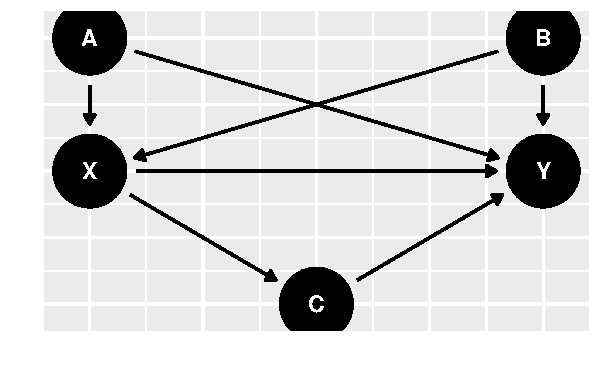
\includegraphics[width=\maxwidth]{figure/backdoor_est_ex-1} 

}

\caption[DAG usado como exemplo para estimar efeito de X em Y]{DAG usado como exemplo para estimar efeito de X em Y.}\label{fig:backdoor_est_ex}
\end{figure}

\end{knitrout}

Considere que o grafo causal é
dado pela \cref{fig:backdoor_est_ex}.
Vamos supor que os dados são gerados da seguinte forma:
$\sigma^2 = 0.01$,
$A \sim N(0, \sigma^2)$, 
$B \sim N(0, \sigma^2)$,
$\epsilon \sim Bernoulli(0.95)$
$X \equiv \I(A + B > 0)\epsilon + \I(A + B < 0)(1-\epsilon)$,
$C \sim N(X, \sigma^2)$, e
$Y \sim N(A + B + C + X, \sigma^2)$:

\begin{knitrout}
\definecolor{shadecolor}{rgb}{0.969, 0.969, 0.969}\color{fgcolor}\begin{kframe}
\begin{alltt}
\hlcom{# Especificar o grafo}
\hlstd{grafo} \hlkwb{<-} \hlstd{dagitty}\hlopt{::}\hlkwd{dagitty}\hlstd{(}\hlstr{"dag \{
    X[e] Y[o]
    \{A B\} -> \{ X Y \}; X -> \{C Y\}; C -> Y \}"}\hlstd{)}

\hlcom{# Simular os dados}
\hlstd{n} \hlkwb{<-} \hlnum{10}\hlopt{^}\hlnum{5}
\hlstd{sd} \hlkwb{=} \hlnum{0.1}
\hlstd{A} \hlkwb{<-} \hlkwd{rnorm}\hlstd{(n,} \hlnum{0}\hlstd{, sd)}
\hlstd{B} \hlkwb{<-} \hlkwd{rnorm}\hlstd{(n,} \hlnum{0}\hlstd{, sd)}
\hlstd{eps} \hlkwb{<-} \hlkwd{rbinom}\hlstd{(n,} \hlnum{1}\hlstd{,} \hlnum{0.8}\hlstd{)}
\hlstd{X} \hlkwb{<-} \hlkwd{as.numeric}\hlstd{(eps}\hlopt{*}\hlstd{((A} \hlopt{+} \hlstd{B)} \hlopt{>} \hlnum{0}\hlstd{)} \hlopt{+}
                  \hlstd{(}\hlnum{1}\hlopt{-}\hlstd{eps)}\hlopt{*}\hlstd{((A} \hlopt{+} \hlstd{B)} \hlopt{<=} \hlnum{0}\hlstd{))}
\hlstd{C} \hlkwb{<-} \hlkwd{rnorm}\hlstd{(n, X, sd)}
\hlstd{Y} \hlkwb{<-} \hlkwd{rnorm}\hlstd{(n, A} \hlopt{+} \hlstd{B} \hlopt{+} \hlstd{C} \hlopt{+} \hlstd{X, sd)}
\hlstd{data} \hlkwb{<-} \hlstd{dplyr}\hlopt{::}\hlkwd{tibble}\hlstd{(A, B, C, X, Y)}
\end{alltt}
\end{kframe}
\end{knitrout}

Estimaremos o efeito causal pela
fórmula do ajuste (\cref{def:ajuste}).
Iniciaremos a análise utilizando $\hmu$ como
sendo uma regressão linear simples:

\begin{knitrout}
\definecolor{shadecolor}{rgb}{0.969, 0.969, 0.969}\color{fgcolor}\begin{kframe}
\begin{alltt}
\hlcom{# Sejam Z variáveis que satisfazem o critério backdoor para}
\hlcom{# estimar o efeito causal de causa em efeito em grafo.}
\hlcom{# Retorna uma fórmula do tipo Y ~ X + Z_1 + ... + Z_d}
\hlstd{fm_ajuste} \hlkwb{<-} \hlkwa{function}\hlstd{(}\hlkwc{grafo}\hlstd{,} \hlkwc{causa}\hlstd{,} \hlkwc{efeito}\hlstd{)}
\hlstd{\{}
  \hlstd{var_backdoor} \hlkwb{<-} \hlstd{dagitty}\hlopt{::}\hlkwd{adjustmentSets}\hlstd{(grafo)[[}\hlnum{1}\hlstd{]]}
  \hlstd{regressores} \hlkwb{=} \hlkwd{c}\hlstd{(causa, var_backdoor)}
  \hlstd{fm} \hlkwb{=} \hlkwd{paste}\hlstd{(regressores,} \hlkwc{collapse} \hlstd{=} \hlstr{"+"}\hlstd{)}
  \hlstd{fm} \hlkwb{=} \hlkwd{paste}\hlstd{(}\hlkwd{c}\hlstd{(efeito, fm),} \hlkwc{collapse} \hlstd{=} \hlstr{"~"}\hlstd{)}
  \hlkwd{as.formula}\hlstd{(fm)}
\hlstd{\}}

\hlcom{# Estima E[Efeito|do(causa = x)] pela }
\hlcom{# formula do ajuste usando mu_chapeu como regressao }
\hlstd{est_do_x_lm} \hlkwb{<-} \hlkwa{function}\hlstd{(}\hlkwc{data}\hlstd{,} \hlkwc{mu_chapeu}\hlstd{,} \hlkwc{causa}\hlstd{,} \hlkwc{x}\hlstd{)}
\hlstd{\{}
  \hlstd{data} \hlopt
    \hlstd{dplyr}\hlopt{::}\hlkwd{mutate}\hlstd{(\{\{causa\}\}} \hlkwb{:=} \hlstd{x)} \hlopt
    \hlkwd{predict}\hlstd{(mu_chapeu,} \hlkwc{newdata} \hlstd{= .)} \hlopt
    \hlkwd{mean}\hlstd{()}
\hlstd{\}}

\hlcom{# Estimação do ACE com regressão linear simples}
\hlstd{fm} \hlkwb{<-} \hlkwd{fm_ajuste}\hlstd{(grafo,} \hlstr{"X"}\hlstd{,} \hlstr{"Y"}\hlstd{)}
\hlstd{mu_chapeu_lm} \hlkwb{<-} \hlkwd{lm}\hlstd{(fm,} \hlkwc{data} \hlstd{= data)}
\hlstd{ace_ajuste_lm} \hlkwb{=} \hlkwd{est_do_x_lm}\hlstd{(data, mu_chapeu_lm,} \hlstr{"X"}\hlstd{,} \hlnum{1}\hlstd{)} \hlopt{-}
  \hlkwd{est_do_x_lm}\hlstd{(data, mu_chapeu_lm,} \hlstr{"X"}\hlstd{,} \hlnum{0}\hlstd{)}
\hlkwd{round}\hlstd{(ace_ajuste_lm)}
\end{alltt}
\begin{verbatim}
## [1] 2
\end{verbatim}
\end{kframe}
\end{knitrout}

Em alguns casos, não é razoável supor que 
$\E[Y|X,\Z]$ é linear. Nestas situações,
é fácil adaptar o código anterior para
algum método não-paramétrico arbitrário.
Exibimos uma implementação usando XGBoost 
\citep{Chen2023}:

\begin{knitrout}
\definecolor{shadecolor}{rgb}{0.969, 0.969, 0.969}\color{fgcolor}\begin{kframe}
\begin{alltt}
\hlkwd{library}\hlstd{(xgboost)}
\hlstd{var_backdoor} \hlkwb{<-} \hlstd{dagitty}\hlopt{::}\hlkwd{adjustmentSets}\hlstd{(grafo,} \hlstr{"X"}\hlstd{,} \hlstr{"Y"}\hlstd{)[[}\hlnum{1}\hlstd{]]}
\hlstd{mu_chapeu} \hlkwb{<-} \hlkwd{xgboost}\hlstd{(}
  \hlkwc{data} \hlstd{= data} \hlopt
    \hlstd{dplyr}\hlopt{::}\hlkwd{select}\hlstd{(}\hlkwd{all_of}\hlstd{(}\hlkwd{c}\hlstd{(var_backdoor,} \hlstr{"X"}\hlstd{)))} \hlopt
    \hlkwd{as.matrix}\hlstd{(),}
  \hlkwc{label} \hlstd{= data} \hlopt
    \hlstd{dplyr}\hlopt{::}\hlkwd{select}\hlstd{(Y)} \hlopt
    \hlkwd{as.matrix}\hlstd{(),}
  \hlkwc{nrounds} \hlstd{=} \hlnum{100}\hlstd{,}
  \hlkwc{objective} \hlstd{=} \hlstr{"reg:squarederror"}\hlstd{,}
  \hlkwc{early_stopping_rounds} \hlstd{=} \hlnum{3}\hlstd{,}
  \hlkwc{max_depth} \hlstd{=} \hlnum{2}\hlstd{,}
  \hlkwc{eta} \hlstd{=} \hlnum{.25}\hlstd{,}
  \hlkwc{verbose} \hlstd{=} \hlnum{FALSE}
\hlstd{)}

\hlstd{est_do_x_xgb} \hlkwb{<-} \hlkwa{function}\hlstd{(}\hlkwc{data}\hlstd{,} \hlkwc{mu_chapeu}\hlstd{,} \hlkwc{causa}\hlstd{,} \hlkwc{x}\hlstd{)}
\hlstd{\{}
  \hlstd{data} \hlopt
    \hlstd{dplyr}\hlopt{::}\hlkwd{mutate}\hlstd{(\{\{causa\}\}} \hlkwb{:=} \hlstd{x)} \hlopt
    \hlstd{dplyr}\hlopt{::}\hlkwd{select}\hlstd{(}\hlkwd{c}\hlstd{(var_backdoor, causa))} \hlopt
    \hlkwd{as.matrix}\hlstd{()} \hlopt
    \hlkwd{predict}\hlstd{(mu_chapeu,} \hlkwc{newdata} \hlstd{= .)} \hlopt
    \hlkwd{mean}\hlstd{()}
\hlstd{\}}

\hlstd{ace_est_xgb} \hlkwb{=} \hlkwd{est_do_x_xgb}\hlstd{(data, mu_chapeu,} \hlstr{"X"}\hlstd{,} \hlnum{1}\hlstd{)} \hlopt{-}
  \hlkwd{est_do_x_xgb}\hlstd{(data, mu_chapeu,} \hlstr{"X"}\hlstd{,} \hlnum{0}\hlstd{)}
\hlkwd{round}\hlstd{(ace_est_xgb,} \hlnum{2}\hlstd{)}
\end{alltt}
\begin{verbatim}
## [1] 2
\end{verbatim}
\end{kframe}
\end{knitrout}

 Como o modelo linear era adequado para $\E[Y|X,\Z]$,
 não vemos diferença entre a estimativa obtida
 pela regressão linear simples e pelo XGBoost.
 Mas será que as estimativas estão adequadas?
 Como simulamos os dados,
 é possível calcular diretamente $\E[Y|do(X=x)]$:
 \begin{align}
  \label{eq:ex_backdoor_1}
  \E[Y|do(X=x)]
  &= \E[\E[Y|X=x, A, B]]
  & \text{\cref{thm:backdoor_ajuste}} \nonumber \\
  &= \E[\E[\E[Y|X=x, A, B, C]|X=x, A, B]]
  & \text{Lei da esperança total} \nonumber \\
  &= \E[\E[A+B+C+X|X=x, A, B]]
  & Y \sim N(A+B+C+X, \sigma^2) \nonumber \\
  &= \E[A + B + 2x]
  & C \sim N(X, \sigma^2) \nonumber \\
  &= 2x
  & \E[A] = \E[B] = 0
 \end{align}
 Uma vez calculado $\E[Y|do(X=x)]$,
 podemos obter o $\ACE$:
 \begin{align*}
  \ACE
  &= \E[Y|do(X=1)] - \E[Y|do(X=0)] \\
  &= 2 \cdot 1 - 2 \cdot 0 = 2
  & \text{\cref{eq:ex_backdoor_1}}
 \end{align*}
 Portanto, as estimativas do $\ACE$ obtidas 
 pela regressão linear e pelo xgboost 
 estão adequadas.
\end{example}

\subsubsection{Ponderação pelo inverso do escore de propensidade (IPW)}

Uma outra forma de estimar 
$\E[Y|do(X=x)]$ e $\E[Y|do(X=x),\Z]$ é
motivada pelo \cref{thm:backdoor_ipw}.
Este resultado determina que, 
se $\Z$ satisfaz a \cref{def:conf_control}, então
\begin{align*}
 \E[Y|do(X=x),\Z] 
 &= \frac{\E\left[Y \I(X=x)|\Z\right]}{f(x|\Z)}.
\end{align*}
Na segunda expressão, $\E[Y \I(X=x)|\Z]$ é 
a regressão de $Y\I(X=x)$ em $\Z$.
Assim, esta quantidade pode ser estimada por
um método de regressão arbitrário, que
denotaremos por $\widehat{\E}[Y \I(X=x)|\Z]$.
Também $f(x|\z)$ é 
usualmente chamado de \textit{escore de propensidade}.
Este escore captura a forma como 
os confundidores atuam sobre $X$
nos dados observacionais.
Como $f$ em geral é desconhecido,
$f(x|\z)$ também o é.
Contudo, quando $X$ é discreto,
podemos estimar $f(x|\z)$ utilizando
algum algoritmo arbitrário de classificação.
Denotaremos esta estimativa por $\hf(x|\z)$.
Se a estimativa for boa, temos
\begin{align*}
 \E[Y|do(X=x),\Z]
 &= \frac{\widehat{\E}[Y \I(X=x)|\Z]}{f(x|\Z)}
 \approx \frac{\widehat{\E}[Y \I(X=x)|\Z]}{\hf(x|\z)}.
\end{align*}

O \cref{thm:backdoor_ipw} também orienta
a estimação de $\E[Y|do(X=x)]$.
Se $\Z$ satisfaz o critério backdoor, então
\begin{align*}
 \E[Y|do(X=x)]
 &= \E\left[\frac{Y \I(X=x)}{f(x|\Z)}\right]
\end{align*}
Como nesta expressão a esperança é
uma média populacional,
ela pode ser aproximada pela média amostral
\begin{align*}
 \E\left[\frac{Y \I(X=x)}{f(x|\Z)}\right]
 &\approx n^{-1} \sum_{i=1}^n \frac{Y_i \I(X_i=x)}{\hf(x|\Z_i)}.
\end{align*}

Combinando estas aproximações, obtemos:
\begin{definition}
 \label{def:ipw}
 Considere que $\Z$ satisfaz a \cref{def:conf_control} e
 $\hf(x|\z)$ é uma estimativa de $f(x|\z)$.
 Os estimadores de $\E[Y|do(X=x),\Z]$ e $\E[Y|do(X=x)]$ 
 por IPW são:
\begin{align*}
 \hdoyzb &:= \frac{\widehat{\E}[Y \I(X=x)|\Z]}{\hf(x|\z)} \\
 \hdoyb &:= n^{-1} \sum_{i=1}^n \frac{Y_i \I(X_i=x)}{\hf(x|\Z_i)}.
\end{align*}
\end{definition}

Se $\hf$ converge para $f$, então sob 
condições relativamente pouco restritivas
$\hdoyb$ converge para $\E[Y|do(X=x)]$.

\begin{theorem}
 \label{thm:conv_ipw}
 Se $\Z$ satisfaz a \cref{def:conf_control}, também
 $\hf$ é invariante a permutações (\cref{def:perm}),
 $\E[|\hf(x|\Z_1)-f(x|\Z_1)|] = o(1)$, e
 existe $M > 0$ tal que
 $\sup_\z \E[|Y| \I(X=x)|\Z=\z] < M$, e
 existe $\delta > 0$ tal que
 $\inf_z \min\{f(x|\Z_1), \hf(x|\Z_1)\} > \delta$, então
 $\hdoyb \convp \E[Y|do(X=x)]$.
\end{theorem}

A seguir, utilizamos novamente dados simulados para
ilustrar a implementação de IPW:

\begin{example}
\label{ex:backdoor_est_ipw}
Considere que o grafo causal e
o modelo de geração dos dados são 
idênticos àqueles do \cref{ex:backdoor_est_ajuste}.
Iniciaremos a análise utilizando 
regressão logística para estimar $\hf$.
 
\begin{knitrout}
\definecolor{shadecolor}{rgb}{0.969, 0.969, 0.969}\color{fgcolor}\begin{kframe}
\begin{alltt}
\hlcom{# Sejam Z variáveis que satisfazem o critério backdoor para}
\hlcom{# estimar o efeito causal de causa em efeito em grafo.}
\hlcom{# Retorna uma fórmula do tipo X ~ Z_1 + ... + Z_d}
\hlstd{fm_ipw} \hlkwb{<-} \hlkwa{function}\hlstd{(}\hlkwc{grafo}\hlstd{,} \hlkwc{causa}\hlstd{,} \hlkwc{efeito}\hlstd{)}
\hlstd{\{}
 \hlstd{var_backdoor} \hlkwb{<-} \hlstd{dagitty}\hlopt{::}\hlkwd{adjustmentSets}\hlstd{(grafo)[[}\hlnum{1}\hlstd{]]}
 \hlstd{fm} \hlkwb{=} \hlkwd{paste}\hlstd{(var_backdoor,} \hlkwc{collapse} \hlstd{=} \hlstr{"+"}\hlstd{)}
 \hlstd{fm} \hlkwb{=} \hlkwd{paste}\hlstd{(}\hlkwd{c}\hlstd{(causa, fm),} \hlkwc{collapse} \hlstd{=} \hlstr{"~"}\hlstd{)}
 \hlkwd{as.formula}\hlstd{(fm)}
\hlstd{\}}

\hlcom{# Estimação do ACE por IPW onde}
\hlcom{# Supomos X binário e}
\hlcom{# f_1 é o vetor P(X_i=1|Z_i)}
\hlstd{ACE_ipw} \hlkwb{<-} \hlkwa{function}\hlstd{(}\hlkwc{data}\hlstd{,} \hlkwc{causa}\hlstd{,} \hlkwc{efeito}\hlstd{,} \hlkwc{f_1}\hlstd{)}
\hlstd{\{}
 \hlstd{data} \hlopt
 \hlkwd{mutate}\hlstd{(}\hlkwc{f_1} \hlstd{= f_1,}
        \hlkwc{est_1} \hlstd{= \{\{efeito\}\}}\hlopt{*}\hlstd{(\{\{causa\}\}}\hlopt{==}\hlnum{1}\hlstd{)}\hlopt{/}\hlstd{f_1,}
        \hlkwc{est_0} \hlstd{= \{\{efeito\}\}}\hlopt{*}\hlstd{(\{\{causa\}\}}\hlopt{==}\hlnum{0}\hlstd{)}\hlopt{/}\hlstd{(}\hlnum{1}\hlopt{-}\hlstd{f_1)}
 \hlstd{)} \hlopt
 \hlkwd{summarise}\hlstd{(}\hlkwc{do_1} \hlstd{=} \hlkwd{mean}\hlstd{(est_1),}
           \hlkwc{do_0} \hlstd{=} \hlkwd{mean}\hlstd{(est_0))} \hlopt
 \hlkwd{mutate}\hlstd{(}\hlkwc{ACE} \hlstd{= do_1} \hlopt{-} \hlstd{do_0)} \hlopt
 \hlstd{dplyr}\hlopt{::}\hlkwd{select}\hlstd{(ACE)}
\hlstd{\}}

\hlstd{fm} \hlkwb{<-} \hlkwd{fm_ipw}\hlstd{(grafo,} \hlstr{"X"}\hlstd{,} \hlstr{"Y"}\hlstd{)}
\hlstd{f_chapeu} \hlkwb{<-} \hlkwd{glm}\hlstd{(fm,} \hlkwc{family} \hlstd{=} \hlstr{"binomial"}\hlstd{,} \hlkwc{data} \hlstd{= data)}
\hlstd{f_1_lm} \hlkwb{<-} \hlkwd{predict}\hlstd{(f_chapeu,} \hlkwc{type} \hlstd{=} \hlstr{"response"}\hlstd{)}
\hlstd{ace_ipw_lm} \hlkwb{<-} \hlstd{data} \hlopt \hlkwd{ACE_ipw}\hlstd{(X, Y, f_1_lm)} \hlopt \hlkwd{as.numeric}\hlstd{()}
\end{alltt}


{\ttfamily\noindent\bfseries\color{errorcolor}{\#\# Error in mutate(., ACE = do\_1 - do\_0): could not find function "{}mutate"{}}}\begin{alltt}
\hlstd{ace_ipw_lm} \hlopt \hlkwd{round}\hlstd{(}\hlnum{2}\hlstd{)}
\end{alltt}


{\ttfamily\noindent\bfseries\color{errorcolor}{\#\# Error in ace\_ipw\_lm \%>\% round(2): object 'ace\_ipw\_lm' not found}}\end{kframe}
\end{knitrout}

Também é fácil adaptar o código acima para
estimar $\ACE$ por IPW utilizando
algum método não-paramétrico para estimar $\hf$.
Abaixo há um exemplo utilizando o XGBoost:

\begin{knitrout}
\definecolor{shadecolor}{rgb}{0.969, 0.969, 0.969}\color{fgcolor}\begin{kframe}
\begin{alltt}
\hlstd{var_backdoor} \hlkwb{<-} \hlstd{dagitty}\hlopt{::}\hlkwd{adjustmentSets}\hlstd{(grafo)[[}\hlnum{1}\hlstd{]]}
\hlstd{f_chapeu} \hlkwb{<-} \hlkwd{xgboost}\hlstd{(}
 \hlkwc{data} \hlstd{= data} \hlopt
   \hlstd{dplyr}\hlopt{::}\hlkwd{select}\hlstd{(}\hlkwd{all_of}\hlstd{(var_backdoor))} \hlopt
   \hlkwd{as.matrix}\hlstd{(),}
 \hlkwc{label} \hlstd{= data} \hlopt
   \hlstd{dplyr}\hlopt{::}\hlkwd{select}\hlstd{(X)} \hlopt
   \hlkwd{as.matrix}\hlstd{(),}
 \hlkwc{nrounds} \hlstd{=} \hlnum{100}\hlstd{,}
 \hlkwc{objective} \hlstd{=} \hlstr{"binary:logistic"}\hlstd{,}
 \hlkwc{early_stopping_rounds} \hlstd{=} \hlnum{3}\hlstd{,}
 \hlkwc{max_depth} \hlstd{=} \hlnum{2}\hlstd{,}
 \hlkwc{eta} \hlstd{=} \hlnum{.25}\hlstd{,}
 \hlkwc{verbose} \hlstd{=} \hlnum{FALSE}
\hlstd{)}

\hlstd{covs} \hlkwb{<-} \hlstd{data} \hlopt \hlstd{dplyr}\hlopt{::}\hlkwd{select}\hlstd{(}\hlkwd{all_of}\hlstd{(var_backdoor))} \hlopt \hlkwd{as.matrix}\hlstd{()}
\hlstd{f_1} \hlkwb{<-} \hlkwd{predict}\hlstd{(f_chapeu,} \hlkwc{newdata} \hlstd{= covs)}
\hlstd{data} \hlopt \hlkwd{ACE_ipw}\hlstd{(X, Y, f_1)} \hlopt \hlkwd{as.numeric}\hlstd{()} \hlopt \hlkwd{round}\hlstd{(}\hlnum{2}\hlstd{)}
\end{alltt}


{\ttfamily\noindent\bfseries\color{errorcolor}{\#\# Error in mutate(., ACE = do\_1 - do\_0): could not find function "{}mutate"{}}}\end{kframe}
\end{knitrout}
\end{example}

\subsubsection{Estimador duplamente robusto}

Os \cref{thm:conv_ajuste,thm:conv_ipw} mostram que,
sob suposições diferentes, 
$\hdoy$ e $\hdoyb$ convergem para $\E[Y|do(X=x)]$.
A ideia do estimador duplamente robusto é
combinar ambos os estimadores de forma
a garantir esta convergência sob 
suposições mais fracas.
Para tal, a ideia por trás do 
estimador duplamente é que
este convirja junto a $\hdoy$ 
quando este é consistente e
para $\hdoyb$ quando aquele o é.

\begin{definition}
 Se $\Z$ satisfaz a \cref{def:conf_control} e 
 sejam $\hf$ e $\hmu$ tais quais nas
 \cref{def:ajuste,def:ipw}.
 O estimador duplamente robusto para
 $\E[Y|do(X=x)]$, $\hdoyc$ é tal que
 \label{def:duplo_robusto}
 \begin{align*}
  \hdoyc 
  &= \hdoy + \hdoyb 
  - \sum_{i=1}^n \frac{\I(X_i=x)\hmu(x,\Z_i)}{n\hat{f}(x|\Z_i)}
 \end{align*}
\end{definition}

O estimador duplamente robusto é consistente para
$\E[Y|do(X=x)]$ tanto sob as condições do
\cref{thm:conv_ajuste} quanto sob as do
\cref{thm:conv_ipw}. A ideia básica é que,
sob as condições do \cref{thm:conv_ajuste},
$\hdoy$ é consistente para $\E[Y|do(X=x)]$ e
$\hdoyb - \sum_{i=1}^n \frac{\I(X_i=x)\hmu(x,\Z_i)}{n\hat{f}(x|\Z_i)}$
converge para $0$. Isto é,
quando $\hdoy$ é consistente,
o estimador duplamente robusto seleciona este termo.
Similarmente, sob as condições do \cref{thm:conv_ipw},
$\hdoyb$ é consistente para $\E[Y|do(X=x)]$ e
$\hdoy - \sum_{i=1}^n \frac{\I(X_i=x)\hmu(x,\Z_i)}{n\hat{f}(x|\Z_i)}$
converge para $0$.

\begin{theorem}
 \label{thm:conv_duplo_robusto}
 Suponha que existe $\epsilon > 0$ tal que
 $\inf_\z \hf(x|\z) > \epsilon$,
 existe $M > 0$ tal que 
 $\sup_\z \hmu(x,\z) < M$, e
 $\hmu$ e $\hf$ são invariantes 
 a permutações (\cref{def:perm}).
 Se as condições do \cref{thm:conv_ajuste} ou
 do \cref{thm:conv_ipw} estão satisfeitas, então
 \begin{align*}
  \hdoyc \convp \E[Y|do(X=x)].
 \end{align*}
\end{theorem}

\begin{example}[Estimador duplamente robusto]
\label{ex:backdoor_est_robusto}
Considere que o grafo causal e
o modelo de geração dos dados são iguais
àqueles descritos no \cref{ex:backdoor_est_ajuste}.
Para implementar o estimador duplamente robusto
combinaremos o estimador da fórmula do ajuste obtido 
por regressão linear no \cref{ex:backdoor_est_ajuste} e
aquele de IPW por regressão logística
no \cref{ex:backdoor_est_ipw}.
\begin{knitrout}
\definecolor{shadecolor}{rgb}{0.969, 0.969, 0.969}\color{fgcolor}\begin{kframe}
\begin{alltt}
\hlstd{mu_1_lm} \hlkwb{<-} \hlstd{data} \hlopt
  \hlstd{dplyr}\hlopt{::}\hlkwd{mutate}\hlstd{(}\hlkwc{X} \hlstd{=} \hlnum{1}\hlstd{)} \hlopt
  \hlkwd{predict}\hlstd{(mu_chapeu_lm,} \hlkwc{newdata} \hlstd{= .)}
\hlstd{mu_0_lm} \hlkwb{<-} \hlstd{data} \hlopt
  \hlstd{dplyr}\hlopt{::}\hlkwd{mutate}\hlstd{(}\hlkwc{X} \hlstd{=} \hlnum{0}\hlstd{)} \hlopt
  \hlkwd{predict}\hlstd{(mu_chapeu_lm,} \hlkwc{newdata} \hlstd{= .)}
\hlstd{corr} \hlkwb{<-} \hlstd{data} \hlopt
  \hlkwd{mutate}\hlstd{(}\hlkwc{mu_1} \hlstd{= mu_1_lm,}
         \hlkwc{mu_0} \hlstd{= mu_0_lm,}
         \hlkwc{f_1} \hlstd{= f_1_lm,}
         \hlkwc{corr_1} \hlstd{= (X} \hlopt{==} \hlnum{1}\hlstd{)}\hlopt{*}\hlstd{mu_1}\hlopt{/}\hlstd{f_1,}
         \hlkwc{corr_0} \hlstd{= (X} \hlopt{==} \hlnum{0}\hlstd{)}\hlopt{*}\hlstd{mu_0}\hlopt{/}\hlstd{(}\hlnum{1}\hlopt{-}\hlstd{f_1))} \hlopt
  \hlkwd{summarise}\hlstd{(}\hlkwc{corr_1} \hlstd{=} \hlkwd{mean}\hlstd{(corr_1),}
            \hlkwc{corr_0} \hlstd{=} \hlkwd{mean}\hlstd{(corr_0))} \hlopt
  \hlkwd{mutate}\hlstd{(}\hlkwc{corr} \hlstd{= corr_1} \hlopt{-} \hlstd{corr_0)} \hlopt
  \hlstd{dplyr}\hlopt{::}\hlkwd{select}\hlstd{(corr)} \hlopt
  \hlkwd{as.numeric}\hlstd{()}
\end{alltt}


{\ttfamily\noindent\bfseries\color{errorcolor}{\#\# Error in mutate(., corr = corr\_1 - corr\_0): could not find function "{}mutate"{}}}\begin{alltt}
\hlstd{ace_rob_lm} \hlkwb{<-} \hlstd{ace_ajuste_lm} \hlopt{+} \hlstd{ace_ipw_lm} \hlopt{-} \hlstd{corr}
\end{alltt}


{\ttfamily\noindent\bfseries\color{errorcolor}{\#\# Error in eval(expr, envir, enclos): object 'ace\_ipw\_lm' not found}}\begin{alltt}
\hlstd{ace_rob_lm} \hlopt \hlkwd{round}\hlstd{(}\hlnum{2}\hlstd{)}
\end{alltt}


{\ttfamily\noindent\bfseries\color{errorcolor}{\#\# Error in ace\_rob\_lm \%>\% round(2): object 'ace\_rob\_lm' not found}}\end{kframe}
\end{knitrout}
\end{example}

\subsection{Exercícios}

\begin{exercise}
 Prove o \cref{lemma:backdoor_random}.
\end{exercise}

\begin{exercise}
 Prove o \cref{lemma:backdoor_pais}.
\end{exercise}

\begin{exercise}
 \label{ex:ace_sem_causa}
 Prove que se $X \notin Anc(Y)$, então $\ACE = 0$.
\end{exercise}

\begin{exercise}
 Prove que a variância amostral satisfaz
 o \cref{def:perm}.
\end{exercise}

\begin{exercise}
 Utilizando como referência o grafo e
 o código no \cref{ex:backdoor_est_ajuste},
 simule dados tais que a estimativa do $\ACE$ é
 diferente quando um método de regressão linear e
 um de regressão não-paramétrica são usados.
\end{exercise}

\subsection{Regression Discontinuity Design (RDD)}

Em determinadas situações,
$X$ é completamente determinado
pelos confundidores, $\Z$ \citep{Lee2010}.
Por exemplo, considere que 
desejamos determinar o efeito causal que
um determinado programa social do governo traz 
sobre o nível de educação dos cidadãos.
Neste caso, $X$ é a indicadora de que
o indíviduo é elegível ao programa e
$Y$ mede o seu nível de educação.
Em alguns casos, é razoável supor que
$X$ é completamente determinado por $Z$,
a renda do indivíduo.

A situação acima traz desafios para
a fórmula do ajuste e IPW discutidos anteriormente.
Primeiramente, como $X = h(\Z)$, 
não é possível estimar $\E[Y|X=x,\Z=\z]$
quando $x \neq h(\z)$.
Portanto, não é possível utilizar
a fórmula do ajuste, uma vez que
ela se baseia na expressão $\E[\E[Y|X=x,\Z]]$.
Similarmente, o estimador de IPW envolve
uma divisão por $f(x|\Z)$.
Assim, quando $x \neq h(\Z)$
há uma divisão por $0$, 
o que torna o estimador indefinido.

\subsubsection{Identificação causal no RDD}

Apesar destas dificuldades,
é possível medir nestas situações
parte do efeito causal de $X$ em $Y$.
Suponha que $\Z \in \Re$ e que 
existe $z_1$ tal que $X = \I(\Z \geq \z_1)$. 
Por exemplo, um benefício pode estar disponível
apenas para cidadãos que tenham renda 
abaixo de um teto ou
uma lei pode ter efeitos
a partir de uma determinada data.

Neste caso, podemos estar interessados em
$\E[Y|do(X=x),\Z=\z_1]$, 
o efeito causal que $X$ tem na 
fronteira de sua implementação.
Intuitivamente, próximo a esta fronteira,
as unidades amostrais são todas similares 
em relação aos confundidores.
Assim, se na fronteira houver uma diferença em $Y$ entre
os valores de $X$, esta diferença 
deve ser decorrente do efeito causal de $X$.
Esta intuição é formalizada no resultado de
identicação causal abaixo:

\begin{theorem}[\citet{Hahn2001}]
 \label{thm:id_rdd}
 Considere que $\Z \in \Re$ satisfaz 
 a \cref{def:conf_control}, $X \in \{0,1\}$, e
 $\E[Y|do(X=0),\Z]$ e $\E[Y|do(X=1),\Z]$ são 
 contínuas em $\Z=\z_1$.
 
 Se $X \equiv \I(\Z \geq \z_1)$, então
 \begin{align*}
  \CACE(\Z=\z_1)
  &= \lim_{\z \downarrow \z_1} \E[Y|\Z = \z] 
  - \lim_{\z \uparrow \z_1} \E[Y|\Z = \z].
 \end{align*}
 
 Se $f(x|\Z) \in (0,1)$ é contínua exceto em $\z_1$, então
 \begin{align*}
  \CACE(\Z=\z_1)
  &= \frac{\lim_{\z \downarrow \z_1} \E[Y|\Z = \z] 
  - \lim_{\z \uparrow \z_1} \E[Y|\Z = \z]}
  {\lim_{\z \downarrow \z_1} f(X=1|\Z=\z) 
  - \lim_{\z \uparrow \z_1} f(X=1|\Z=\z)}.
 \end{align*}
\end{theorem}

Um detalhe sutil do \cref{thm:id_rdd} é que
$X \equiv \I(\Z > \z_1)$ não é
o suficiente para termos certeza que
$\Z$ satisfaz o critério backdoor.
Por exemplo, considere que 
o governo criasse um benefício fiscal para
todas empresas sediadas em um determinado município.
Neste caso, a ocorrência do benefício é
função da sede da empresa. 
Contudo, a relação causal é mais complexa.
Se o benefício for suficientemente alto,
poderia motivar empresas a 
moverem sua sede para o município.
Em outras palavras, 
o benefício seria causa da localização da sede e não o contrário.
Neste caso, não seria possível aplicar o \cref{thm:id_rdd}.
Este tipo de raciocínio indica que a análise por RDD é
mais efetiva quando é difícil interferir sobre o valor de $\Z$.
Por exemplo, como um indivíduo não pode interferir sobre a sua idade,
é mais fácil justificar o uso de RDD em
uma campanha de vacinação em que
apenas indivíduos acima de uma determinada idade são vacinados.

Um outro ponto importante de interpretação do \cref{thm:id_rdd} é que,
embora $\E[Y|do(X=0),\Z]$ e $\E[Y|do(X=1),\Z]$ sejam supostas contínuas,
$f(X=1|\Z)$ e $\E[Y|\Z]$ não o são. Intuitivamente,
podemos imaginar $X$ representa a indicadora de que
uma determinada política é adotada.
Por exemplo, podemos imaginar que $X$ indica que um indivíduo foi vacinado,
$\Z$ a sua idade e $Y$ a sua hospitalização.
Neste caso, $\E[Y|do(X=0),\Z]$ e $\E[Y|do(X=1),\Z]$ representam
a taxa de hospitalização quando
todos os indivíduos são vacinados ou
quando todos eles não o são.
Nestas situações, seria razoável supor que
a taxa de hospitalização é contínua em função da idade, pois
não esperamos que exista uma grande descontinuidade 
nas condições de saúde entre
indivíduos com $69$ e com $70$ anos de idade.
Este tipo de conclusão muitas vezes é resumido pela expressão em latim
\textit{natura non facit saltus}
(a natureza não faz saltos).
Por outro lado, nos dados observados,
a política não é adotada para uma faixa de valores de $\Z$ e
passa a ser adotada a partir de um ponto,
o que é responsável pela descontinuidade em
$\E[Y|\Z]$ e em $f(X=1|\Z)$.
Podemos imaginar que a vacinação é empregada 
somente em indivíduos com mais de $70$ anos.
Esta descontinuidade na política humana cria
uma diferença importante entre indivíduos
com $69$ e com $70$ anos,
o que explica uma diferença grande 
nas taxas de hospitalização entre estas idades
nos dados observados.

\subsubsection{Estimação no RDD}

O \cref{thm:id_rdd} indica que $\CACE(\Z=\z_1)$ é
função da regressão de $Y$ sobre $\Z$, $\E[Y|\Z]$, e
sobre o classificador, $f(X=1|\Z)$.
Uma possível estratégia é estimarmos 
estas quantidades separadamente e, a seguir,
estimarmos o $\CACE$ trocando
as quantias populacionais pelas quantias estimadas.

Uma dificuldade nesta estratégia é que
sabemos que $\E[Y|\Z]$ e $f(X=1|\Z)$ são discontínuas.
Para lidar com esta dificuldade, 
uma possibilidade é 
realizar uma regressão para $\Z < \z_1$ e
outra para $\Z \geq \z_1$.

\begin{definition}
 \label{def:est_rdd}
 Seja $D_{<} = \{i: \Z_i < \z_1\}$
 o conjunto de unidades amostrais em que $\Z_i < \z_1$,
 $\widehat{\E}_{<}[Y|\Z]$ e $\hf_{<}(X=1|\Z)$ regressões ajustadas
 utilizando apenas dados em $D_{<}$ e
 $\widehat{\E}_{\geq}[Y|\Z]$ e $\hf_{\geq}(X=1|\Z)$ ajustadas
 em $D^{c}_{<}$.
 O estimador RDD para $\CACE(\z_1)$ é
 \begin{align*}
  \hCACE(\z_1)
  := \frac{\widehat{\E}_{\geq}[Y|\z_1] - \widehat{\E}_{<}[Y|\z_1]}
  {\hf_{\geq}(X=1|\Z) - \hf_{<}(X=1|\Z)}.
 \end{align*}
 Em particular, se sabemos a priori que
 $f(X=1|\z) = 1$ para $\z \geq \z_1$ e
 $f(X=1|\z) = 0$ para $\z < \z_1$, então
 \begin{align*}
  \hCACE(\z_1)
  := \widehat{\E}_{\geq}[Y|\z_1] - \widehat{\E}_{<}[Y|\z_1]
 \end{align*}
\end{definition}

O exemplo a seguir ilustra a implementação de RDD quando
$X \equiv \I(\Z \geq \z_1)$ utilizando 
tanto regressão linear quanto 
regressão de Kernel de Nadaraya-Watson.

\begin{example}
 \label{ex:rdd}
 Considere que $Z_i$ satisfaz 
 o critério backdoor para estimar 
 o efeito causal de $X$ em $Y$.
 Além disso, $Z_i \sim N(0,1)$,
 $X_i \equiv \I(Z_i \geq 0)$ e
 $Y_i|X_i,Z_i \sim N(50(X_i+1)(Z_i + 1), 1)$.
 Podemos simular os dados da seguinte forma:
 
\begin{knitrout}
\definecolor{shadecolor}{rgb}{0.969, 0.969, 0.969}\color{fgcolor}\begin{kframe}
\begin{alltt}
\hlstd{n} \hlkwb{<-} \hlnum{1000}
\hlstd{Z} \hlkwb{<-} \hlkwd{rnorm}\hlstd{(n)}
\hlstd{X} \hlkwb{<-} \hlstd{Z} \hlopt{>=} \hlnum{0}
\hlstd{Y} \hlkwb{<-} \hlkwd{rnorm}\hlstd{(n,} \hlnum{50}\hlopt{*}\hlstd{(X}\hlopt{+}\hlnum{1}\hlstd{)}\hlopt{*}\hlstd{(Z}\hlopt{+}\hlnum{1}\hlstd{))}
\hlstd{data} \hlkwb{<-} \hlkwd{tibble}\hlstd{(X, Y, Z)}
\end{alltt}


{\ttfamily\noindent\bfseries\color{errorcolor}{\#\# Error in tibble(X, Y, Z): could not find function "{}tibble"{}}}\begin{alltt}
\hlkwd{plot}\hlstd{(Z, Y)}
\end{alltt}
\end{kframe}\begin{figure}[t]

{\centering 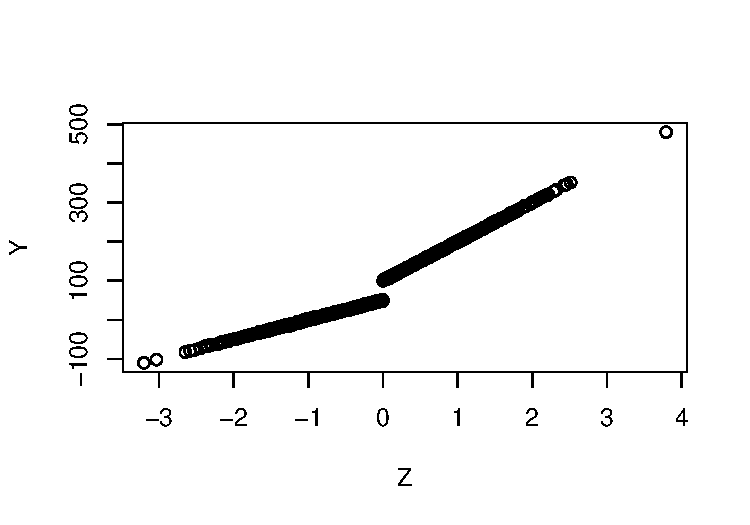
\includegraphics[width=\maxwidth]{figure/rdd_ex_1_1-1} 

}

\caption[Exemplo em que Z satisfaz o critério backdoor para medir o efeito causal de X em Y e X = I(Z $>$ 0)]{Exemplo em que Z satisfaz o critério backdoor para medir o efeito causal de X em Y e X = I(Z $>$ 0). Como resultado da descontinuidade da propensidade de X em Z = 0, há uma descontinuidade na regressão de Y em Z no ponto Z=0.}\label{fig:rdd_ex_1_1}
\end{figure}

\end{knitrout}
 
 Como estamos simulando os dados,
 podemos calcular $\CACE(0)$:
 \begin{align*}
  \CACE(0) 
  &= \lim_{\z \downarrow 0}\E[Y|\Z=\z] 
  - \lim_{\z \uparrow 0}\E[Y|\Z=\z]
  & \text{\cref{thm:id_rdd}} \\
  &= \lim_{\z \downarrow 0}\E[Y|X=1,\Z=\z]
  - \lim_{\z \uparrow 0}\E[Y|X=0,\Z=\z] \\
  &= \lim_{\z \downarrow 0} 50(1+1)(\z+1)
  - \lim_{\z \uparrow 0} 50(0+1)(\z+1)
  = 50
 \end{align*}
\end{example}

O código abaixo estima $\CACE(0)$ usando regressão linear:

\begin{knitrout}
\definecolor{shadecolor}{rgb}{0.969, 0.969, 0.969}\color{fgcolor}\begin{kframe}
\begin{alltt}
\hlstd{regs} \hlkwb{=} \hlstd{data} \hlopt
  \hlkwd{mutate}\hlstd{(}\hlkwc{Z1} \hlstd{= (Z} \hlopt{>=} \hlnum{0}\hlstd{))} \hlopt
  \hlkwd{group_by}\hlstd{(Z1)} \hlopt
  \hlkwd{summarise}\hlstd{(}
    \hlkwc{intercepto} \hlstd{=} \hlkwd{lm}\hlstd{(Y} \hlopt{~} \hlstd{Z)}\hlopt{$}\hlstd{coefficients[}\hlnum{1}\hlstd{],}
    \hlkwc{coef_angular} \hlstd{=} \hlkwd{lm}\hlstd{(Y} \hlopt{~} \hlstd{Z)}\hlopt{$}\hlstd{coefficients[}\hlnum{2}\hlstd{]}
  \hlstd{)}
\end{alltt}


{\ttfamily\noindent\bfseries\color{errorcolor}{\#\# Error in summarise(., intercepto = lm(Y \textasciitilde{} Z)\$coefficients[1], coef\_angular = lm(Y \textasciitilde{} : could not find function "{}summarise"{}}}\begin{alltt}
\hlstd{regs}
\end{alltt}


{\ttfamily\noindent\bfseries\color{errorcolor}{\#\# Error in eval(expr, envir, enclos): object 'regs' not found}}\begin{alltt}
\hlstd{est_cace} \hlkwb{=} \hlnum{1}\hlopt{*}\hlstd{regs[}\hlnum{2}\hlstd{,} \hlnum{2}\hlstd{]} \hlopt{+} \hlnum{0}\hlopt{*}\hlstd{regs[}\hlnum{2}\hlstd{,} \hlnum{3}\hlstd{]} \hlopt{-}
  \hlnum{1}\hlopt{*}\hlstd{regs[}\hlnum{1}\hlstd{,} \hlnum{2}\hlstd{]} \hlopt{+} \hlnum{0}\hlopt{*}\hlstd{regs[}\hlnum{1}\hlstd{,} \hlnum{3}\hlstd{]}
\end{alltt}


{\ttfamily\noindent\bfseries\color{errorcolor}{\#\# Error in eval(expr, envir, enclos): object 'regs' not found}}\begin{alltt}
\hlkwd{round}\hlstd{(}\hlkwd{as.numeric}\hlstd{(est_cace),} \hlnum{2}\hlstd{)}
\end{alltt}


{\ttfamily\noindent\bfseries\color{errorcolor}{\#\# Error in eval(expr, envir, enclos): object 'est\_cace' not found}}\end{kframe}
\end{knitrout}

Similarmente, podemos estimar $\CACE(0)$ usando
regressão por kernel de Nadaraya-Watson:

\begin{knitrout}
\definecolor{shadecolor}{rgb}{0.969, 0.969, 0.969}\color{fgcolor}\begin{kframe}
\begin{alltt}
\hlkwd{library}\hlstd{(np)}
\hlkwd{options}\hlstd{(}\hlkwc{np.messages} \hlstd{=} \hlnum{FALSE}\hlstd{)}
\hlstd{nw_reg} \hlkwb{<-} \hlkwa{function}\hlstd{(}\hlkwc{data}\hlstd{,} \hlkwc{valor}\hlstd{)}
\hlstd{\{}
  \hlstd{bw} \hlkwb{<-} \hlkwd{npregbw}\hlstd{(}\hlkwc{xdat} \hlstd{= data}\hlopt{$}\hlstd{Z,} \hlkwc{ydat} \hlstd{= data}\hlopt{$}\hlstd{Y)}\hlopt{$}\hlstd{bw}
  \hlkwd{npksum}\hlstd{(}\hlkwc{txdat}\hlstd{= data}\hlopt{$}\hlstd{Z,} \hlkwc{exdat} \hlstd{= valor,} \hlkwc{tydat} \hlstd{= data}\hlopt{$}\hlstd{Y,} \hlkwc{bws} \hlstd{= bw)}\hlopt{$}\hlstd{ksum}\hlopt{/}
    \hlkwd{npksum}\hlstd{(}\hlkwc{txdat} \hlstd{= data}\hlopt{$}\hlstd{Z,} \hlkwc{exdat} \hlstd{= valor,} \hlkwc{bws} \hlstd{= bw)}\hlopt{$}\hlstd{ksum}
\hlstd{\}}

\hlstd{reg_baixo} \hlkwb{<-} \hlstd{data} \hlopt
  \hlkwd{filter}\hlstd{(Z} \hlopt{<} \hlnum{0}\hlstd{)} \hlopt
  \hlkwd{nw_reg}\hlstd{(}\hlnum{0}\hlstd{)}
\end{alltt}


{\ttfamily\noindent\bfseries\color{errorcolor}{\#\# Error in `filter()`:\\\#\# i In argument: `Z < 0`.\\\#\# Caused by error:\\\#\# ! `..1` must be of size 100000 or 1, not size 1000.}}\begin{alltt}
\hlstd{reg_cima} \hlkwb{<-} \hlstd{data} \hlopt
  \hlkwd{filter}\hlstd{(Z} \hlopt{>=} \hlnum{0}\hlstd{)} \hlopt
  \hlkwd{nw_reg}\hlstd{(}\hlnum{0}\hlstd{)}
\end{alltt}


{\ttfamily\noindent\bfseries\color{errorcolor}{\#\# Error in `filter()`:\\\#\# i In argument: `Z >= 0`.\\\#\# Caused by error:\\\#\# ! `..1` must be of size 100000 or 1, not size 1000.}}\begin{alltt}
\hlstd{est_cace} \hlkwb{<-} \hlstd{reg_cima} \hlopt{-} \hlstd{reg_baixo}
\end{alltt}


{\ttfamily\noindent\bfseries\color{errorcolor}{\#\# Error in eval(expr, envir, enclos): object 'reg\_cima' not found}}\begin{alltt}
\hlkwd{round}\hlstd{(est_cace,} \hlnum{2}\hlstd{)}
\end{alltt}


{\ttfamily\noindent\bfseries\color{errorcolor}{\#\# Error in eval(expr, envir, enclos): object 'est\_cace' not found}}\end{kframe}
\end{knitrout}

\subsection{Exercícios}

\begin{exercise}
 Crie um exemplo em que,
 ao contrário do \cref{ex:rdd},
 $\E[Y|X=1,\Z]$ não é linear em $\Z$.
 Compare as estimativas de $\CACE$ usando
 a regressão linear e 
 algum método de regressão não-paramétrica.
\end{exercise}
